% --- LaTeX Homework Template - S. Venkatraman ---

% --- Set document class and font size ---

\documentclass[letterpaper, 11pt]{article}

% --- Package imports ---

\usepackage{
  amsmath, amsthm, amssymb, mathtools, dsfont,	  % Math typesetting
  graphicx, wrapfig, subfig, float,                  % Figures and graphics formatting
  listings, color, inconsolata, pythonhighlight,     % Code formatting
  fancyhdr, sectsty, hyperref, enumerate, enumitem, caption } % Headers/footers, section fonts, links, lists

% --- Page layout settings ---

% Set page margins
\usepackage[left=1.35in, right=1.35in, bottom=1in, top=1.1in, headsep=0.2in]{geometry}

% Anchor footnotes to the bottom of the page
\usepackage[bottom]{footmisc}
% Set line spacing
\renewcommand{\baselinestretch}{1.2}

% Set spacing between paragraphs
\setlength{\parskip}{1.5mm}

% Allow multi-line equations to break onto the next page
\allowdisplaybreaks

% Enumerated lists: make numbers flush left, with parentheses around them
\setlist[enumerate]{wide=0pt, leftmargin=21pt, labelwidth=0pt, align=left}
\setenumerate[1]{label={(\arabic*)}}

% --- Page formatting settings ---

% Set link colors for labeled items (blue) and citations (red)
\hypersetup{colorlinks=true, linkcolor=blue, citecolor=red}

% Make reference section title font smaller
\renewcommand{\refname}{\large\bf{References}}

% --- Settings for printing computer code ---

% Define colors for green text (comments), grey text (line numbers),
% and green frame around code
\definecolor{greenText}{rgb}{0.5, 0.7, 0.5}
\definecolor{greyText}{rgb}{0.5, 0.5, 0.5}
\definecolor{codeFrame}{rgb}{0.5, 0.7, 0.5}

% Define code settings
\lstdefinestyle{code} {
  frame=single, rulecolor=\color{codeFrame},            % Include a green frame around the code
  numbers=left,                                         % Include line numbers
  numbersep=8pt,                                        % Add space between line numbers and frame
  numberstyle=\tiny\color{greyText},                    % Line number font size (tiny) and color (grey)
  commentstyle=\color{greenText},                       % Put comments in green text
  basicstyle=\linespread{1.1}\ttfamily\footnotesize,    % Set code line spacing
  keywordstyle=\ttfamily\footnotesize,                  % No special formatting for keywords
  showstringspaces=false,                               % No marks for spaces
  xleftmargin=1.95em,                                   % Align code frame with main text
  framexleftmargin=1.6em,                               % Extend frame left margin to include line numbers
  breaklines=true,                                      % Wrap long lines of code
  postbreak=\mbox{\textcolor{greenText}{$\hookrightarrow$}\space} % Mark wrapped lines with an arrow
}

% Set all code listings to be styled with the above settings
\lstset{style=code}

% --- Math/Statistics commands ---

% Add a reference number to a single line of a multi-line equation
% Usage: "\numberthis\label{labelNameHere}" in an align or gather environment
\newcommand\numberthis{\addtocounter{equation}{1}\tag{\theequation}}

% Shortcut for bold text in math mode, e.g. $\b{X}$
\let\b\mathbf

% Shortcut for bold Greek letters, e.g. $\bg{\beta}$
\let\bg\boldsymbol

% Shortcut for calligraphic script, e.g. %\mc{M}$
\let\mc\mathcal

% \mathscr{(letter here)} is sometimes used to denote vector spaces
\usepackage[mathscr]{euscript}

% Convergence: right arrow with optional text on top
% E.g. $\converge[w]$ for weak convergence
\newcommand{\converge}[1][]{\xrightarrow{#1}}

% Normal distribution: arguments are the mean and variance
% E.g. $\normal{\mu}{\sigma}$
\newcommand{\normal}[2]{\mathcal{N}\left(#1,#2\right)}

% Uniform distribution: arguments are the left and right endpoints
% E.g. $\unif{0}{1}$
\newcommand{\unif}[2]{\text{Uniform}(#1,#2)}

% Independent and identically distributed random variables
% E.g. $ X_1,...,X_n \iid \normal{0}{1}$
\newcommand{\iid}{\stackrel{\smash{\text{iid}}}{\sim}}

% Equality: equals sign with optional text on top
% E.g. $X \equals[d] Y$ for equality in distribution
\newcommand{\equals}[1][]{\stackrel{\smash{#1}}{=}}

% Math mode symbols for common sets and spaces. Example usage: $\R$
\newcommand{\R}{\mathbb{R}}   % Real numbers
\newcommand{\C}{\mathbb{C}}   % Complex numbers
\newcommand{\Q}{\mathbb{Q}}   % Rational numbers
\newcommand{\Z}{\mathbb{Z}}   % Integers
\newcommand{\N}{\mathbb{N}}   % Natural numbers
\newcommand{\F}{\mathcal{F}}  % Calligraphic F for a sigma algebra
\newcommand{\El}{\mathcal{L}} % Calligraphic L, e.g. for L^p spaces

% Math mode symbols for probability
\newcommand{\pr}{\mathbb{P}}    % Probability measure
\newcommand{\E}{\mathbb{E}}     % Expectation, e.g. $\E(X)$
\newcommand{\var}{\text{Var}}   % Variance, e.g. $\var(X)$
\newcommand{\cov}{\text{Cov}}   % Covariance, e.g. $\cov(X,Y)$
\newcommand{\corr}{\text{Corr}} % Correlation, e.g. $\corr(X,Y)$
\newcommand{\B}{\mathcal{B}}    % Borel sigma-algebra

% Other miscellaneous symbols
\newcommand{\tth}{\text{th}}	% Non-italicized 'th', e.g. $n^\tth$
\newcommand{\Oh}{\mathcal{O}}	% Big-O notation, e.g. $\O(n)$
\newcommand{\1}{\mathds{1}}	% Indicator function, e.g. $\1_A$

% Additional commands for math mode
\DeclareMathOperator*{\argmax}{argmax}    % Argmax, e.g. $\argmax_{x\in[0,1]} f(x)$
\DeclareMathOperator*{\argmin}{argmin}    % Argmin, e.g. $\argmin_{x\in[0,1]} f(x)$
\DeclareMathOperator*{\spann}{Span}       % Span, e.g. $\spann\{X_1,...,X_n\}$
\DeclareMathOperator*{\bias}{Bias}        % Bias, e.g. $\bias(\hat\theta)$
\DeclareMathOperator*{\ran}{ran}          % Range of an operator, e.g. $\ran(T) 
\DeclareMathOperator*{\dv}{d\!}           % Non-italicized 'with respect to', e.g. $\int f(x) \dv x$
\DeclareMathOperator*{\diag}{diag}        % Diagonal of a matrix, e.g. $\diag(M)$
\DeclareMathOperator*{\trace}{trace}      % Trace of a matrix, e.g. $\trace(M)$

% Numbered theorem, lemma, etc. settings - e.g., a definition, lemma, and theorem appearing in that 
% order in Section 2 will be numbered Definition 2.1, Lemma 2.2, Theorem 2.3. 
% Example usage: \begin{theorem}[Name of theorem] Theorem statement \end{theorem}
\theoremstyle{definition}
\newtheorem{theorem}{Theorem}[section]
\newtheorem{proposition}[theorem]{Proposition}
\newtheorem{lemma}[theorem]{Lemma}
\newtheorem{corollary}[theorem]{Corollary}
\newtheorem{definition}[theorem]{Definition}
\newtheorem{example}[theorem]{Example}
\newtheorem{remark}[theorem]{Remark}

% Un-numbered theorem, lemma, etc. settings
% Example usage: \begin{lemma*}[Name of lemma] Lemma statement \end{lemma*}
\newtheorem*{theorem*}{Theorem}
\newtheorem*{proposition*}{Proposition}
\newtheorem*{lemma*}{Lemma}
\newtheorem*{corollary*}{Corollary}
\newtheorem*{definition*}{Definition}
\newtheorem*{example*}{Example}
\newtheorem*{remark*}{Remark}
\newtheorem*{claim}{Claim}

% --- Left/right header text (to appear on every page) ---

% Include a line underneath the header, no footer line
\pagestyle{fancy}
\renewcommand{\footrulewidth}{0pt}
\renewcommand{\headrulewidth}{0.4pt}

% Left header text: course name/assignment number
\lhead{CSE 5245 (Intro to Network Science) -- Lab 1}

% Right header text: your name
\rhead{Raman Ebrahimi}

% --- Document starts here ---

\begin{document}
\subsection*{Code explanation}

\paragraph{}To begin with, after reading data from the local cloud in Google Colaboratory, we had three functions defined to simplify the computation process. The first of three serves the purpose of computing centrality measures using predefined functions in NetworkX; the other two are for plotting and visualizing for better analysis; the first provides a heat map for each centrality measure, and the second one plots a histogram for each centrality measure.

\begin{lstlisting}[language=python, caption={Functions for future computations}, label={lst:Pycode}]
from networkx.classes.function import is_directed
def centrality_measures(g):
    d_cent = nx.degree_centrality(g) # this is normalized by default
    c_cent = nx.closeness_centrality(g) # this is normalized by default
    b_cent = nx.betweenness_centrality(g)
    e_cent = nx.eigenvector_centrality(g)
    h_cent = nx.harmonic_centrality(g)
    pr = nx.pagerank(g) # alpha is 0.85 by default, we can change it.
    clus_coeff = nx.clustering(g)
    # these are all dictionaries from nodes to their centrality value (or other variables).
    if nx.is_directed(g):
      in_cent = nx.in_degree_centrality(g)
      out_cent = nx.out_degree_centrality(g)
    else:
      in_cent = 0
      out_cent = 0
      
    return d_cent, c_cent, b_cent, e_cent, h_cent, pr, clus_coeff, in_cent, out_cent

def draw(G, pos, measures, measure_name):
    
    nodes = nx.draw_networkx_nodes(G, pos, node_size=2, cmap=plt.cm.plasma, 
                                   node_color=list(measures.values()),
                                   nodelist=measures.keys())
    nodes.set_norm(mcolors.SymLogNorm(linthresh=0.01, linscale=1, base=10))
    edges = nx.draw_networkx_edges(G, pos)

    plt.title(measure_name)
    plt.colorbar(nodes)
    plt.axis('off')
    plt.savefig(measure_name+'.png', format='png')
    plt.show()


def plot_hist(measure, measure_name):
    plt.hist(list(measure.values()))
    plt.title(measure_name)
    # plt.axis('off')
    plt.savefig(measure_name+'hist.png', format='png')
    plt.show()\end{lstlisting}
\newpage
\subsection*{Dataset 1: General Relativity and Quantum Cosmology collaboration network}
\paragraph{}The first dataset was General Relativity and Quantum Cosmology collaboration network dataset or as it is referred to in the code:  GrQc.
\paragraph{}After trying to compute the radius, center, diameter, and eccentricity and getting errors giving infinity values, we discovered that our network was disconnected.
\paragraph{Degree Centrality}Then, the defined functions were used to compute centralities. The first centrality is Degree Centrality. As shown in figure~\ref{fig:d_cent} histogram, most degree centralities are close to zero, and only a few are nearly 0.01. 
\begin{figure}[h]
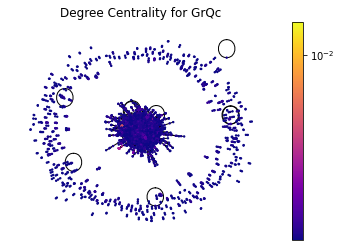
\includegraphics[width=0.5\textwidth]{GrQc_d_cent.png}
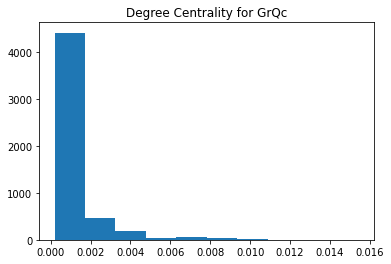
\includegraphics[width=0.5\textwidth]{GrQc_d_cent_hist.png}
\captionsetup{justification=centering,margin=0.5cm}
\caption{Heatmap for degree centrality and an approximate visualization of the network (on the left). Histogram of degree centrality of the nodes (on the right).}
\label{fig:d_cent}
\end{figure}
Since we are using a normalized measure, the highest possible centrality, meaning if we had a node connected to every other node, is 1. So we can conclude that our network is far from a complete graph, and we can say it's sparse.
\paragraph{Closeness Centrality}The next measured centrality, closeness centrality, scores each node based on its sum of shortest paths. 
\begin{figure}[h]
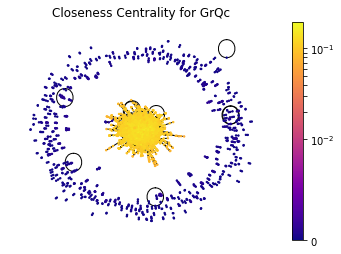
\includegraphics[width=0.5\textwidth]{GrQc_c_cent.png}
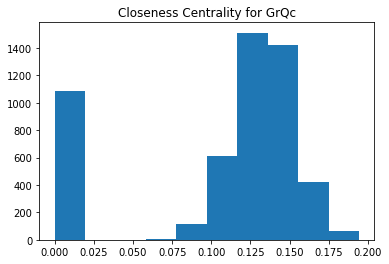
\includegraphics[width=0.5\textwidth]{GrQc_c_cent_hist.png}
\captionsetup{justification=centering,margin=0.5cm}
\caption{Heatmap for closeness centrality and an approximate network visualization (on the left). Histogram of closeness centrality of the nodes (on the right).}
\label{fig:c_cent}
\end{figure}
As seen in the figure~\ref{fig:c_cent}, the distribution of closeness centrality is much more different from degree centrality. The histogram consists of some nodes whose closeness centrality is near zero and some with normal-like distribution with a mean near ~0.14. \\
By looking at the heatmap, we can see what this means, some nodes in the middle are almost similarly close to each other, and there is a ring around these nodes with low closeness centrality meaning they're much further from each other than the ones in the middle.
\paragraph{Betweenness Centrality}counts the number of times a node lies on the shortest paths between other nodes. We can see in the figure~\ref{fig:b_cent} that the same thing happened to degree centrality is happening here as well. Most nodes have near zero betweenness centrality, and few are higher than 0.015. 
\begin{figure}[h]
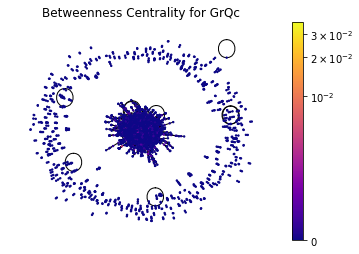
\includegraphics[width=0.5\textwidth]{GrQc_b_cent.png}
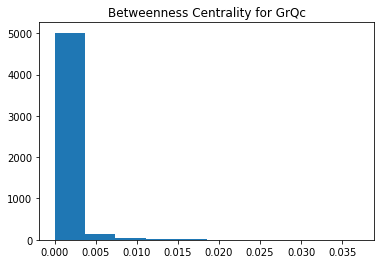
\includegraphics[width=0.5\textwidth]{GrQc_b_cent_hist.png}
\captionsetup{justification=centering,margin=0.5cm}
\caption{Heatmap for betweenness centrality and an approximate network visualization (on the left). Histogram of betweenness centrality of the nodes (on the right).}
\label{fig:b_cent}
\end{figure}
Combining the results from the last two measures, we have some nodes that are relatively close to each other, but those same nodes are not on many shortest paths and are not important in this way.
\paragraph{Eigenvector Centrality}can identify nodes with influence over the whole network, not just those directly connected to it. With this explanation, we could expect the output of the code, and seeing figure~\ref{fig:e_cent} confirms our expectations.
\begin{figure}[h]
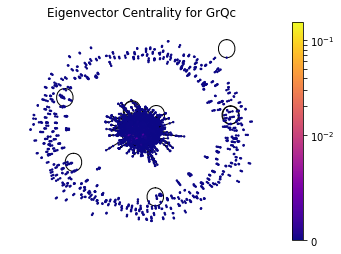
\includegraphics[width=0.5\textwidth]{GrQc_e_cent.png}
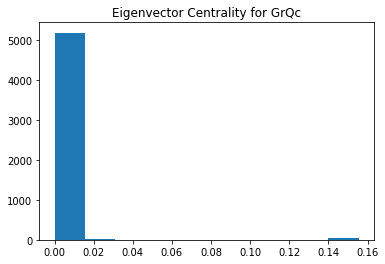
\includegraphics[width=0.5\textwidth]{GrQc_e_cent_hist.png}
\captionsetup{justification=centering,margin=0.5cm}
\caption{Heatmap for eigenvector centrality and an approximate network visualization (on the left). Histogram of eigenvector centrality of the nodes (on the right).}
\label{fig:e_cent}
\end{figure}
\paragraph{PageRank}uncovers nodes whose influence extends beyond their direct connections into the wider network. This measure is useful in directed networks, and since our network is not directed, we may not be able to see this measure's full potential here. 
\begin{figure}[h]
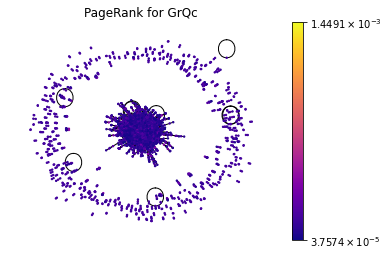
\includegraphics[width=0.5\textwidth]{GrQc_pr.png}
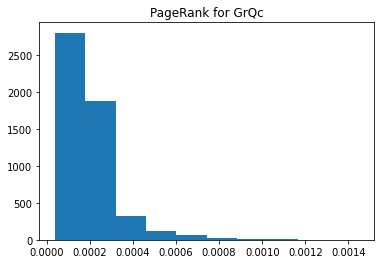
\includegraphics[width=0.5\textwidth]{GrQc_pr_hist.png}
\captionsetup{justification=centering,margin=0.5cm}
\caption{Heatmap for PageRank and an approximate network visualization (on the left). Histogram of PageRank of the nodes (on the right).}
\label{fig:pr}
\end{figure}
On the histogram of PageRank, non-similar to betweenness and eigenvector centralities, its curve is not as steep as it was on former measures. 
\paragraph{Clustering Coefficient} And lastly, a clustering coefficient measures the degree to which nodes in a graph tend to cluster together. Looking at the heatmap in figure~\ref{fig:clustering}, we can see that nodes with clustering coefficient in the middle part are more than nodes with high cluster coefficient in the ring.
\begin{figure}[h]
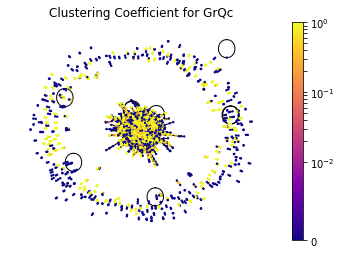
\includegraphics[width=0.5\textwidth]{GrQc_clustering.png}
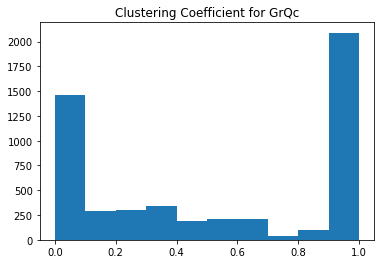
\includegraphics[width=0.5\textwidth]{GrQc_clustering_hist.png}
\captionsetup{justification=centering,margin=0.5cm}
\caption{Heatmap for clustering coefficient and an approximate network visualization (on the left). Histogram of clustering coefficient of the nodes (on the right).}
\label{fig:clustering}
\end{figure}
Also, since there are not many connections on the ring, we can say that there are high clustering coefficients because some packs of fully connected nodes, such as two or three nodes connected, make their clustering coefficient equal to one. 
\paragraph{Further measurements}There were some other measures computed, which are visible in the code, that are worth mentioning. We had 48,260 triangles, and with 5242 nodes, the total possible triangles were 23,993,367,880, meaning very few triangles were formed in the network. Moreover, there were bridges in the network (obviously), and the largest connected component was visualized in the middle of every figure up until now. \\
We had 4158 nodes in the largest connected component, which is close to \%80 of the nodes, and we had 13428 edges in the largest connected component, which is around \%92 of the total edges of the network. This means the nodes outside the largest connected component are barely connected, as we mentioned before.
\paragraph{NOTE}From the next section on, we will only talk about more general measurements of networks in hand; however, we will still include visualizations in a folder named "Figures," and we will briefly talk about them.
%--------------------------------------------------------------------------------------------------------------------------------------------------------------
%--------------------------------------------------------------------------------------------------------------------------------------------------------------
%--------------------------------------------------------------------------------------------------------------------------------------------------------------
\newpage
%--------------------------------------------------------------------------------------------------------------------------------------------------------------
%--------------------------------------------------------------------------------------------------------------------------------------------------------------
%--------------------------------------------------------------------------------------------------------------------------------------------------------------
\subsection*{Dataset 2: Wikipedia vote network}
\paragraph{}This section's network is a directed network where a directed edge from node i to node j represents that user i voted on user j.
\paragraph{}Since visualization of the graph for this part takes a long time, I decided to skip that step and only use the metric and measurements plus histograms without knowing how the network looks. This situation can happen for many real-life networks since our datasets are getting bigger and bigger, and we will have to understand the structure and behavior of networks with minimum computation cost.
\paragraph{Analysis using metrics}We know we have a directed graph and by trying to compute normal diameter we know our network is disconnected since we get the error "Found infinite path length because the digraph is not strongly connected." We used a new way of computing diameter which ignored infinity values.
\begin{equation}
diameter:\;\; 10
\end{equation}
Moreover, we computed both largest weakly and strongly components, and computed the fraction of nodes and edges in thes components:
\begin{equation}
\begin{split} 
nodes\; in\; the\; largest\; weakly\; connected\; component:\;\; 0.9931131412508785 \\
edges\; in\; the\; largest\; weakly\; connected\; component:\;\; 0.9997492501615408 \\
nodes\; in\; the\; largest\; strongly\; connected\; component:\;\; 0.18271257905832747 \\
edges\; in\; the\; largest\; strongly\; connected\; component:\;\; 0.3805225240864508 \\
\end{split}
\end{equation}
These numbers tell us that almost every node is in the largest weakly connected component which consists almost every edge in our network. Therefore there are few nodes that are connected to each other outside this component that makes this graph disconnected. On the other hand, we have a relatively small largest strongly connected component which means most of the nodes in our weakly sonnected component are on the edge of our network.
\paragraph{Analysis using histograms}We can also get some insights from seeing the distribution of centralities and histograms. Looking at histograms, we see some similarities with out first dataset. In the histograms we can see similar shapes in closeness and harmonic centralities, as expected, and also we see very low betweenness centrality for all nodes which means all of our nodes are similarly not on many shortest paths. There are some high clustering coefficients which are for mentioned disconnected nodes, and lastly, we have low PageRank for all the nodes which means we don't have nodes with many incoming links and we can confirm this by looking at in-degree centrality histogram.
%--------------------------------------------------------------------------------------------------------------------------------------------------------------
%--------------------------------------------------------------------------------------------------------------------------------------------------------------
%--------------------------------------------------------------------------------------------------------------------------------------------------------------
\newpage
%--------------------------------------------------------------------------------------------------------------------------------------------------------------
%--------------------------------------------------------------------------------------------------------------------------------------------------------------
%--------------------------------------------------------------------------------------------------------------------------------------------------------------
\subsection*{Dataset 3: Gnutella peer-to-peer network, August 8 2002}
\paragraph{}For this part we got both histograms and shape of our network plus heatmap, same as first dataset, but we mostly talk about general metrics and briefly mention what we can get from histograms and heatmap, such as similarities and differences.
\paragraph{Analysis using metrics}Same as last section, we have a directed network, and we computed same measures as last section.
\begin{equation}
\begin{split} 
nodes\; in\; the\; largest\; weakly\; connected\; component:\;\; 0.999682590065069 \\
edges\; in\; the\; largest\; weakly\; connected\; component:\;\; 0.9999518698560909 \\
nodes\; in\; the\; largest\; strongly\; connected\; component:\;\; 0.3282018727186161 \\
edges\; in\; the\; largest\; strongly\; connected\; component:\;\; 0.4482360302257304 \\
\end{split}
\end{equation}
Looking at these fractions and comparing them to WikiVote dataset, we can say this network has both larger strongly and weakly connected components. They both contain higher percentage of nodes and edges. But still, very few nodes are making our network disconnected, and the difference in strongly and weakly connected components tell us that many nodes are still on the edge of graph but graph is more connected in comparison with WikiVote network.
\paragraph{}Some other measures were calculated for strongly connected component which are worth mentioning:
\begin{equation}
\begin{split} 
radius\; of\; largest\; strongly\; connected\; component\; is:\;\; 12 \\
diameter\; of\; largest\; strongly\; connected\; component\; is:\;\; 19
\end{split}
\end{equation}
These results don't agree with the information given on the SNAP website which might be because of how the diameter and radius are calculated within directed graphs.
\paragraph{Analysis using histograms}The most interesting histogram for this section is the closeness centrality histogram. For this network, most of the nodes have non-zero closeness centrality which means the average shortest path from a node to every other node follows an almost normal distribution.
%--------------------------------------------------------------------------------------------------------------------------------------------------------------
%--------------------------------------------------------------------------------------------------------------------------------------------------------------
%--------------------------------------------------------------------------------------------------------------------------------------------------------------
\newpage
%--------------------------------------------------------------------------------------------------------------------------------------------------------------
%--------------------------------------------------------------------------------------------------------------------------------------------------------------
%--------------------------------------------------------------------------------------------------------------------------------------------------------------
\subsection*{Dataset 4: Social circles: Facebook}
\paragraph{Analysis using metrics and figures}For this part, we have a connected, undirected graph with 1,612,010 triangles. Since we have 4039 nodes in the network, most possible number of triangles are 10,973,563,139 which means we have a reasonable amount of triangles. Also, we can see that graph has bridges and we have extracted them in a dictionary since these bridges can be important. It's worth mentioning that we had bridges in previous networks too, but since they were representing nodes which were connected only to each other, they weren't as important, or in the same way important, as bridges for this part are.
\paragraph{}We also computed diameter and radius of networks:
\begin{equation}
\begin{split} 
radius\; :\;\; 4 \\
diameter\;:\;\; 8
\end{split}
\end{equation}
Which means the largest shortest path in our graph is 8 and we can get to any node at most in 8 steps. Moreover, using figure~\ref{fig:fb} we can see that our networks has communities. Here we don't see much difference in the histograms but we do have communities and clusters in the network. The reason this is not showing up in the clustering coefficient histogram is that these communities have almost similar clustering coefficients which the will shape a similar histogram to other datasets.
\begin{figure}[h]
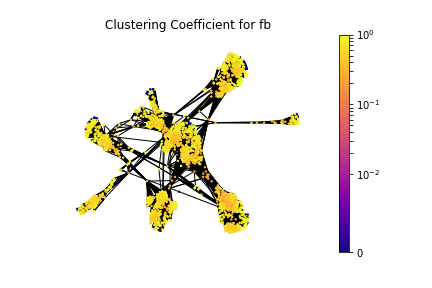
\includegraphics[width=0.5\textwidth]{fb_clustering.png}
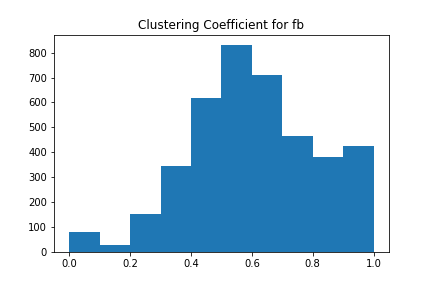
\includegraphics[width=0.5\textwidth]{fb_clustering_hist.png}
\captionsetup{justification=centering,margin=0.5cm}
\caption{Heatmap for clustering coefficient and an approximate network visualization (on the left). Histogram of clustering coefficient of the nodes (on the right).}
\label{fig:fb}
\end{figure}
Also, we tried to find and visualise communities in the graph using Girvan-Newman algorithm but the computational cost of this algorithm is massive! Therefore, we decided to skip this step.






% --- Bibliography ---

% Start a bibliography with two items, a book and a webpage.
% To include a citation, use "\cite{book1}".

\begin{thebibliography}{2}

\bibitem{Networks, Crowds, and Markets: Reasoning about a Highly Connected World}
  Easley, David; Kleinberg Jon.
  \textit{Networks, Crowds, and Markets: Reasoning about a Highly Connected World}.
  Cambridge University Press, 2010.
  Print.

\bibitem{webpage1}
  ``Stanford Network Analysis Project''.
  SNAP, Stanford.
  Online. 
  \texttt{http://snap.stanford.edu/index.html}
  
  
\bibitem{webpage1}
  ``Network Analysis in Python''.
  NetworkX.
  Online. 
  \texttt{https://networkx.org/documentation/stable/reference/introduction.html}

\end{thebibliography}

% --- Document ends here ---

\end{document}